\section{随机试验}
\textbf{定义}：对随机现象的观察，称为\textbf{随机试验}（简称试验），记为 $E$。

\textbf{特点}：
\begin{enumerate}
	\item 可在相同条件下重复进行。
	\item 试验结果可能不止一个，但能明确所有的可能结果。
	\item 试验前无法确定是哪个结果会出现。
\end{enumerate}

\section{样本空间、随机事件}
\textbf{样本空间（$\Omega$）}：试验的所有可能结果所组成的集合，记为 $\Omega = \{\omega\}$。

\textbf{样本点（$\omega$）}：试验的每一个结果或样本空间的每个元素。

\textbf{随机事件（事件）}：试验中可能出现也可能不出现的情况，记作 $A, B, C$ 等。任何事件均对应着样本空间的某个\textbf{子集}。

\textbf{特殊事件}：
\begin{itemize}
	\item \textbf{必然事件}：样本空间 $\Omega$。
	\item \textbf{不可能事件}：空集 $\emptyset$。
	\item \textbf{基本事件}：只包含一个样本点的事件 $\{\omega\}$。
\end{itemize}

\textbf{事件间的关系}：
\begin{enumerate}
	\item \textbf{包含关系}：$A \subset B$（$A$ 发生必导致 $B$ 发生）。
	\item \textbf{和事件}：事件 $A$ 与 $B$ 至少有一个发生 $\Leftrightarrow$ $A \cup B$ 发生。
	\item \textbf{积事件}：$A$ 与 $B$ 同时发生 $\Leftrightarrow$ $A \cap B = AB$ 发生。
	\item \textbf{差事件}：$A - B$ 发生 $\Leftrightarrow$ 事件 $A$ 发生而事件 $B$ 不发生。
	\item \textbf{互斥的事件}：$AB = \emptyset$。
	\item \textbf{互逆的事件}：若 $A \cup B = \Omega$，且 $AB = \emptyset$，称 $A$ 与 $B$ 互为逆事件。表示 $A, B$ 不可能同时发生，但必有一个发生。
\end{enumerate}

\subsection{事件的运算}
\textbf{1. 交换律（Commutative Law）}
\begin{itemize}
	\item $A \cup B = B \cup A$
	\item $AB = BA$（注：$AB$ 通常表示交集 $A \cap B$）
\end{itemize}

\textbf{2. 结合律（Associative Law）}
\begin{itemize}
	\item $(A \cup B) \cup C = A \cup (B \cup C)$
	\item $(AB)C = A(BC)$
\end{itemize}

\textbf{3. 分配律（Distributive Law）}
\begin{itemize}
	\item $(A \cup B)C = (AC) \cup (BC)$
	\item $(AB) \cup C = (A \cup C)(B \cup C)$
\end{itemize}

\textbf{4. 对偶律 / 德·摩根定律（De Morgan's Laws）}：这是集合运算中非常重要的变换规则，描述了"补集"与"并、交运算"的关系。
\begin{itemize}
	\item \textbf{基本形式}：
	\begin{itemize}
		\item $\overline{A \cup B} = \bar{A} \cap \bar{B}$（并的补等于补的交）
		\item $\overline{AB} = \bar{A} \cup \bar{B}$（交的补等于补的并）
	\end{itemize}
	\item \textbf{可推广形式（Generalization）}：
	\begin{itemize}
		\item $\overline{\bigcup_{k} A_k} = \bigcap_{k} \bar{A}_k$
		\item $\overline{\bigcap_{k} A_k} = \bigcup_{k} \bar{A}_k$
	\end{itemize}
\end{itemize}

\textcolor{blue}{例1}（掷骰子）：$E_4$：掷一颗骰子，考察可能出现的点数。
\begin{itemize}
	\item 样本空间：$S_4 = \{1, 2, 3, 4, 5, 6\}$。
	\item 事件 $A =$"掷出偶数点" $= \{2, 4, 6\}$。
	\item 事件 $B =$"掷出大于4的点"。
\end{itemize}

\section{古典概型与概率}
\textbf{概率的性质}：
\begin{enumerate}
	\item $P(\emptyset) = 0$。
	\item \textbf{有限可加性}：设 $A_1, \ldots, A_n$ 是 $n$ 个两两互不相容的事件（$A_i A_j = \emptyset$），则
	\begin{equation}
		P(A_1 \cup A_2 \cup \ldots \cup A_n) = P(A_1) + P(A_2) + \ldots + P(A_n)
		\label{eq:第一章:有限可加性}
	\end{equation}
	\item \textbf{事件差}：$P(A - B) = P(A) - P(AB)$。
	\item \textbf{加法公式}：对任意两事件 $A, B$，有
	\begin{equation}
		P(A \cup B) = P(A) + P(B) - P(AB)
		\label{eq:第一章:加法公式}
	\end{equation}
	\item \textbf{互补性}：$P(\bar{A}) = 1 - P(A)$。
\end{enumerate}

\textcolor{blue}{例}（古典概型抽球公式）：盒中有 $N$ 个球，其中 $M$ 个白球，现从中任抽 $n$ 个球，则这 $n$ 个球中恰有 $k$ 个白球的概率是：
\begin{equation}
	P = \frac{C_{M}^{k} C_{N-M}^{n-k}}{C_{N}^{n}}
	\label{eq:第一章:抽球公式}
\end{equation}

\section{条件概率、独立性}
\textbf{条件概率（定义）}：设 $A, B$ 为两个事件，且 $P(A) > 0$，则称 $B$ 在 $A$ 发生的条件下发生的概率为
\begin{equation}
	P(B|A) = \frac{P(AB)}{P(A)}
	\label{eq:第一章:条件概率}
\end{equation}
\textbf{乘法公式（推导）}：$P(AB) = P(A)\,P(B|A)$。

\textbf{两个事件的独立性}：若 $P(AB) = P(A)\,P(B)$，则称事件 $A$ 与 $B$ 相互独立。

\textcolor{blue}{例}（独立性证明）：证明若 $A, B$ 相互独立，则 $A, \bar{B}$ 相互独立。
\begin{proof}
	由事件差公式
	\begin{equation}
		P(A\bar{B}) = P(A - AB) = P(A) - P(AB)
		\label{eq:第一章:独立性证明1}
	\end{equation}
	因 $A, B$ 独立：$P(AB) = P(A)P(B)$，故
	\begin{equation}
		P(A\bar{B}) = P(A) - P(A)P(B) = P(A)\big[1 - P(B)\big] = P(A)P(\bar{B})
		\label{eq:第一章:独立性证明2}
	\end{equation}
	因此 $A$ 与 $\bar{B}$ 相互独立。
\end{proof}

\section{全概率公式与贝叶斯公式}
\textbf{全概率公式（应用例题）}：\textcolor{blue}{例1}（袋子抽球）：甲袋（2白，1红），乙袋（2红，1白）。从甲袋中任取一球放入乙袋，再从乙袋任取一球是红球（$B$）的概率。
\begin{itemize}
	\item 设 $A_1$——从甲袋放入乙袋的是白球（$P(A_1) = 2/3$）；$A_2$——从甲袋放入乙袋的是红球（$P(A_2) = 1/3$）。
	\item 若 $A_1$ 发生（乙袋 2白2红），$P(B|A_1) = 2/4 = 1/2$。
	\item 若 $A_2$ 发生（乙袋 1白3红），$P(B|A_2) = 3/4$。
	\item \textbf{全概率公式}：$P(B) = P(B|A_1)P(A_1) + P(B|A_2)P(A_2)$
	\begin{equation}
		P(B) = \frac{2}{4} \cdot \frac{2}{3} + \frac{3}{4} \cdot \frac{1}{3} = \frac{4}{12} + \frac{3}{12} = \frac{7}{12}
		\label{eq:第一章:全概率例题}
	\end{equation}
\end{itemize}

\textbf{贝叶斯公式}：
\begin{equation}
	P(A_j|B) = \frac{P(A_j)P(B|A_j)}{\sum_{i=1}^{n} P(A_i)P(B|A_i)}, \quad (j=1,\dots,n)
	\label{eq:第一章:贝叶斯公式}
\end{equation}

\section{错题}
概率为 0 的事件不一定是不可能事件。（选 D）

\begin{center}
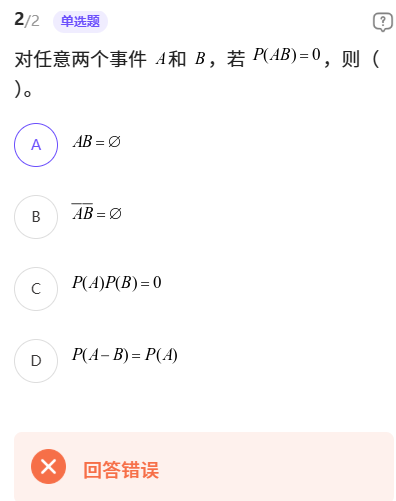
\includegraphics[width=0.5\linewidth]{Figures/prob_1.png}
\end{center}

\begin{center}

\includegraphics[width=0.5\linewidth]{Figures/prob_2.png}
\end{center}
